% CVPR 2025 Paper Template; see https://github.com/cvpr-org/author-kit

\documentclass[10pt,twocolumn,letterpaper]{article}

%%%%%%%%% PAPER TYPE  - PLEASE UPDATE FOR FINAL VERSION
\usepackage{cvpr}              % To produce the CAMERA-READY version
%\usepackage[review]{cvpr}      % To produce the REVIEW version
% \usepackage[pagenumbers]{cvpr} % To force page numbers, e.g. for an arXiv version

% Import additional packages in the preamble file, before hyperref
%
% --- inline annotations
%
\newcommand{\red}[1]{{\color{red}#1}}
\newcommand{\todo}[1]{{\color{red}#1}}
\newcommand{\TODO}[1]{\textbf{\color{red}[TODO: #1]}}
% --- disable by uncommenting  
% \renewcommand{\TODO}[1]{}
% \renewcommand{\todo}[1]{#1}



% It is strongly recommended to use hyperref, especially for the review version.
% hyperref with option pagebackref eases the reviewers' job.
% Please disable hyperref *only* if you encounter grave issues, 
% e.g. with the file validation for the camera-ready version.
%
% If you comment hyperref and then uncomment it, you should delete *.aux before re-running LaTeX.
% (Or just hit 'q' on the first LaTeX run, let it finish, and you should be clear).
\definecolor{cvprblue}{rgb}{0.21,0.49,0.74}
\usepackage[pagebackref,breaklinks,colorlinks,allcolors=cvprblue]{hyperref}

%%%%%%%%% PAPER ID  - PLEASE UPDATE
\def\paperID{*****} % *** Enter the Paper ID here
\def\confName{CVPR}
\def\confYear{2025}

%%%%%%%%% TITLE - PLEASE UPDATE
\title{Powerlifting Vision}

%%%%%%%%% AUTHORS - PLEASE UPDATE
\author{Hunter M. Von Tungeln\\
{\tt\small hvt7@hawaii.edu}
% For a paper whose authors are all at the same institution,
% omit the following lines up until the closing ``}''.
% Additional authors and addresses can be added with ``\and'',
% just like the second author.
% To save space, use either the email address or home page, not both
\and
Tyler Mak\\
{\tt\small tylermak@hawaii.edu}
\and
Benjamin Banilower \\
{\tt\small bbanilow@hawaii.edu}\\
\and 
University of Hawaii at Manoa\\
2500 Campus Rd.\\
Honolulu, HI 96822
}

\begin{document}
\maketitle
\begin{abstract}
Powerlifting is a sport consisting of three main barbell lifts, the squat, the bench press, and the deadlift. For each movement, there are three attempts to perform. All three of these movements are judged by three judges, two on the sides, and one in the front. These lifts must be performed to a certain standard in order to be called a ``good lift." This paper examines the barbell squat and seeks to utilize existing computer vision technology to judge squat depth. For a squat to be considered ``depth" in Powerlifting, the hip crease must be below the top of the knee. To do this, recent pose estimation models are used to generate pose estimations from videos of a human squatting, as well as key points corresponding to joints and other body parts. The pose estimation video output and key points are then fed into a trained neural network that predicts if a squat meets the depth standard. We demonstrate that our simple framework is effective in judging squat depth, with [add remarks about data here]. \\
\end{abstract}    
\section{Introduction}
\label{sec:intro}
Pose estimation is a fundamental problem in computer vision and artificial intelligence, with many applications. The way pose estimation is done is predicting locations of key points, like joints in a given video. Human 3D pose estimation aims to predict and map key points from a 2D video into 3D space. In the last decade, there have been multiple models developed that aim to solve this problem. This paper is an application of this solution to another problem, being judging in the sport of Powerlifting. 
\subsection{Powerlifting Background}
Powerlifting is a sport consisting of three main barbell lifts, the squat, the bench press, and the deadlift. For each movement, there are three attempts to perform. All three of these movements are judged by three judges, two on the sides, and one in the front. These lifts must be performed to a certain standard in order to be called a ``good lift." Judges will either give a white light for a good lift, or a red light for a lift that is no-good. To be counted as a good lift, a lifter must receive at least two white lights from the judges. If a lifter receives at least one white-light, they may contest the judge's decisions. The main rule that we are concerned with for the purpose of this paper is the squat depth rule, where the hip crease must reach below the top of the knee joint at the bottom of the squat movement. 

\subsection{Motivation}
Sometimes, judging in Powerlifting can be subjective, because it is the perception of the judges that counts.  An innattentive or unfocused judge may not see if the lift was performed to the set standard, and may very well red-light a good lift, and vice-versa. It is possible that a seasoned judge may also make a bad call, and red-light a good lift, or white-light a bad lift. The motivation behind this project is to make judging lifts at a powerlifting meet more objective than subjective, which can be achieved with the use of computer vision technology. 
\begin{figure}[t]
  \centering
  %\fbox{\rule{0pt}{2in} \rule{0.9\linewidth}{0pt}}
   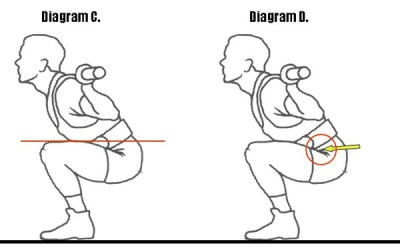
\includegraphics[width=0.8\linewidth]{squat-depth.jpg}

   \caption{Diagram of a squat considered to be ``depth."}
   \label{fig:onecol}
\end{figure}


%-------------------------------------------------------------------------
\section{Related Work}
\label{sec:relatedwork}
As stated before, there have been many models developed for the purpose of 3D human pose estimation. Such models include PoseFormer, Detectron2, VideoPose3D, and PETR-Pose. [Remarks about their performance from their specific papers here]. For this problem, it is not of interest to reinvent 3D pose estimation models, but rather to apply them to a specific, niche problem. We are interested in how the output from these models can be used in determining squat depth in Powerlifting. 

%-------------------------------------------------------------------------
%\subsection{References}

%List and number all bibliographical references in 9-point Times, single-spaced, at the end of your paper.
%When referenced in the text, enclose the citation number in square brackets, for
%example~\cite{Authors14}.

\section{Data And Collection}
\label{sec:formatting}
\subsection{Data Collection}
The data for this project consisted of barbell squat videos with a single person in focus. A single frame was manually extracted from each video. Videos for this paper was collected through publicly available videos on Instagram and YouTube, as well as from friends of the authors. Videos were cropped to isolate the person squatting. The dataset included squat videos from multiple people at different angles in order to make our decision making model more robust. A total of 230 videos were collected for this project, with one frame per video being used for the dataset. 
\subsection{Pre-Processing}
To preprocess, frames were renamed, indexed, and given an  ``Is Depth" attribute, annotated with a default boolean false value. Frames were then manually annotated by one author, Hunter, as he is an experienced powerlifter with a lot of informal experience of judging squat depth. This information was stored in a CSV file, with the index, frame path, and Is Depth as columns. These frames were then fed into our pose estimation model, provided by Google's MediaPipe, to generate landmarks.  
\subsection{Landmarks and Pose Estimation}
When a frame is fed into the pose estimation model provided by Google's MediaPipe, an annotated image was generated, and two sets of landmarks for body locations were generated. The first set is a list of landmarks relative to locations within the image, while the second set is a list of landmarks of real-world positions in 3D space. Each landmark has a corresponding x-coordinate, y-coordinate, and z-coordinate, resulting in 99 numeric data points in each set of landmark, for a total of 198 numeric points for each frame. These values were stored in CSV files, with each column corresponding to the the specific landmarks and their respective x, y, and z values, along with paths to the original frame, the annotated image, and the Is Depth attribute. One CSV file contained only the image landmarks, another contained only the world landmarks, and the third contained both.

%-------------------------------------------------------------------------


\section{Methods and Experiments}
\label{sec:formatting}
In this section, we present multiple frameworks for judging Powerlifting squat depth.
\subsection{Comparison Test}
Comparing output coordinates, world and image (hunter or ben can do this)
\subsection{Multi-Layer Perceptron}
Leveraging the three different datasets from the output of Mediapipe's pose landmark detection algorithm, we use a MLP classifier from sklearn to judge squat depth for a variety of images.The features and labels are prepared by removing unnecessary columns and selecting the target labels. A hyperparameter grid is defined to tune the MLP classifier's hidden layer sizes, learning rates, and L2 regularization. Stratified k-fold cross-validation ensures balanced class distribution. Multiple random states are tested to evaluate model robustness, with stratified splitting maintaining class balance during training, validation, and testing to ensure that the small size of the data does not heavily skew performance metrics. Standard scaling is applied to standardize features, improving convergence. GridSearchCV is used to find the best hyperparameters, and the optimal MLP model is trained and evaluated on validation and test sets.
\subsection{Convolutional Neural Network}
Using a Convolutional Neural Network on a set of squat images, annotated with a boolean if it is depth or not, we first preprocessed the data by normalizing the pixel values by dividing the pixel values into the range of [\0,1] as neural networks perform better on normalized input. The data is split into a 60/20/20 split before being converted to numpy arrays. A model is then created using Keras. The architecture includes:
  Three convolutional layers with increasing filter sizes (32, 64, 128), each followed by max pooling.
  A flattening layer to convert 2D data into a 1D vector.
  A fully connected dense layer with 128 units and ReLU activation.
  A dropout layer with a 50\% dropout rate to prevent overfitting.
  An output dense layer with a sigmoid activation for binary classification
The model is then compiled using the Adam optimizer, binary cross-entropy loss, and accuracy as the metric used to evaluate performance. Given the limitation of having a small dataset, anymore than three convolutional layers in the architecture results in overfitting of the training data, resulting in 0.5 accuracy on the test data.

%-------------------------------------------------------------------------


\section{Results}
\label{sec:results}
[Insert how our model performed on our given data, remark on why it performed the way it did]
\subsection{Comparison Test}
Hunter or Ben
\subsection{Multi-Layer Perceptron}
Tyler
\subsection{Convolutional Neural Network}
Tyler
%-------------------------------------------------------------------------


\section{Conclusion}
\label{sec:conclusion}
[Insert remarks on our solution, how our solution can be improved, areas for future use and improvement]

%-------------------------------------------------------------------------


%\section{Final copy}

You must include your signed IEEE copyright release form when you submit your finished paper.
We MUST have this form before your paper can be published in the proceedings.

Please direct any questions to the production editor in charge of these proceedings at the IEEE Computer Society Press:
\url{https://www.computer.org/about/contact}.
%{
%    \small
%    \bibliographystyle{ieeenat_fullname}
%    \bibliography{main}
%}

% WARNING: do not forget to delete the supplementary pages from your submission 
% \clearpage
\setcounter{page}{1}
\maketitlesupplementary


\section{Rationale}
\label{sec:rationale}
% 
Having the supplementary compiled together with the main paper means that:
% 
\begin{itemize}
\item The supplementary can back-reference sections of the main paper, for example, we can refer to \cref{sec:intro};
\item The main paper can forward reference sub-sections within the supplementary explicitly (e.g. referring to a particular experiment); 
\item When submitted to arXiv, the supplementary will already included at the end of the paper.
\end{itemize}
% 
To split the supplementary pages from the main paper, you can use \href{https://support.apple.com/en-ca/guide/preview/prvw11793/mac#:~:text=Delete%20a%20page%20from%20a,or%20choose%20Edit%20%3E%20Delete).}{Preview (on macOS)}, \href{https://www.adobe.com/acrobat/how-to/delete-pages-from-pdf.html#:~:text=Choose%20%E2%80%9CTools%E2%80%9D%20%3E%20%E2%80%9COrganize,or%20pages%20from%20the%20file.}{Adobe Acrobat} (on all OSs), as well as \href{https://superuser.com/questions/517986/is-it-possible-to-delete-some-pages-of-a-pdf-document}{command line tools}.

\end{document}
